
%% bare_jrnl.tex
%% V1.3
%% 2007/01/11
%% by Michael Shell
%% see http://www.michaelshell.org/
%% for current contact information.
%%
%% This is a skeleton file demonstrating the use of IEEEtran.cls
%% (requires IEEEtran.cls version 1.7 or later) with an IEEE journal paper.
%%
%% Support sites:
%% http://www.michaelshell.org/tex/ieeetran/
%% http://www.ctan.org/tex-archive/macros/latex/contrib/IEEEtran/
%% and
%% http://www.ieee.org/



% *** Authors should verify (and, if needed, correct) their LaTeX system  ***
% *** with the testflow diagnostic prior to trusting their LaTeX platform ***
% *** with production work. IEEE's font choices can trigger bugs that do  ***
% *** not appear when using other class files.                            ***
% The testflow support page is at:
% http://www.michaelshell.org/tex/testflow/


%%*************************************************************************
%% Legal Notice:
%% This code is offered as-is without any warranty either expressed or
%% implied; without even the implied warranty of MERCHANTABILITY or
%% FITNESS FOR A PARTICULAR PURPOSE! 
%% User assumes all risk.
%% In no event shall IEEE or any contributor to this code be liable for
%% any damages or losses, including, but not limited to, incidental,
%% consequential, or any other damages, resulting from the use or misuse
%% of any information contained here.
%%
%% All comments are the opinions of their respective authors and are not
%% necessarily endorsed by the IEEE.
%%
%% This work is distributed under the LaTeX Project Public License (LPPL)
%% ( http://www.latex-project.org/ ) version 1.3, and may be freely used,
%% distributed and modified. A copy of the LPPL, version 1.3, is included
%% in the base LaTeX documentation of all distributions of LaTeX released
%% 2003/12/01 or later.
%% Retain all contribution notices and credits.
%% ** Modified files should be clearly indicated as such, including  **
%% ** renaming them and changing author support contact information. **
%%
%% File list of work: IEEEtran.cls, IEEEtran_HOWTO.pdf, bare_adv.tex,
%%                    bare_conf.tex, bare_jrnl.tex, bare_jrnl_compsoc.tex
%%*************************************************************************

% Note that the a4paper option is mainly intended so that authors in
% countries using A4 can easily print to A4 and see how their papers will
% look in print - the typesetting of the document will not typically be
% affected with changes in paper size (but the bottom and side margins will).
% Use the testflow package mentioned above to verify correct handling of
% both paper sizes by the user's LaTeX system.
%
% Also note that the "draftcls" or "draftclsnofoot", not "draft", option
% should be used if it is desired that the figures are to be displayed in
% draft mode.
%
\documentclass[journal]{IEEEtran}
%
% If IEEEtran.cls has not been installed into the LaTeX system files,
% manually specify the path to it like:
% \documentclass[journal]{../sty/IEEEtran}





% Some very useful LaTeX packages include:
% (uncomment the ones you want to load)


% *** MISC UTILITY PACKAGES ***
%
%\usepackage{ifpdf}
% Heiko Oberdiek's ifpdf.sty is very useful if you need conditional
% compilation based on whether the output is pdf or dvi.
% usage:
% \ifpdf
%   % pdf code
% \else
%   % dvi code
% \fi
% The latest version of ifpdf.sty can be obtained from:
% http://www.ctan.org/tex-archive/macros/latex/contrib/oberdiek/
% Also, note that IEEEtran.cls V1.7 and later provides a builtin
% \ifCLASSINFOpdf conditional that works the same way.
% When switching from latex to pdflatex and vice-versa, the compiler may
% have to be run twice to clear warning/error messages.






% *** CITATION PACKAGES ***
%
\usepackage{cite}
% cite.sty was written by Donald Arseneau
% V1.6 and later of IEEEtran pre-defines the format of the cite.sty package
% \cite{} output to follow that of IEEE. Loading the cite package will
% result in citation numbers being automatically sorted and properly
% "compressed/ranged". e.g., [1], [9], [2], [7], [5], [6] without using
% cite.sty will become [1], [2], [5]--[7], [9] using cite.sty. cite.sty's
% \cite will automatically add leading space, if needed. Use cite.sty's
% noadjust option (cite.sty V3.8 and later) if you want to turn this off.
% cite.sty is already installed on most LaTeX systems. Be sure and use
% version 4.0 (2003-05-27) and later if using hyperref.sty. cite.sty does
% not currently provide for hyperlinked citations.
% The latest version can be obtained at:
% http://www.ctan.org/tex-archive/macros/latex/contrib/cite/
% The documentation is contained in the cite.sty file itself.






% *** GRAPHICS RELATED PACKAGES ***
%
\ifCLASSINFOpdf
  % \usepackage[pdftex]{graphicx}
  % declare the path(s) where your graphic files are
  % \graphicspath{{../pdf/}{../jpeg/}}
  % and their extensions so you won't have to specify these with
  % every instance of \includegraphics
  % \DeclareGraphicsExtensions{.pdf,.jpeg,.png}
\else
  % or other class option (dvipsone, dvipdf, if not using dvips). graphicx
  % will default to the driver specified in the system graphics.cfg if no
  % driver is specified.
   \usepackage[dvips]{graphicx}
  % declare the path(s) where your graphic files are
  % \graphicspath{{../eps/}}
  % and their extensions so you won't have to specify these with
  % every instance of \includegraphics
  % \DeclareGraphicsExtensions{.eps}
\fi
% graphicx was written by David Carlisle and Sebastian Rahtz. It is
% required if you want graphics, photos, etc. graphicx.sty is already
% installed on most LaTeX systems. The latest version and documentation can
% be obtained at: 
% http://www.ctan.org/tex-archive/macros/latex/required/graphics/
% Another good source of documentation is "Using Imported Graphics in
% LaTeX2e" by Keith Reckdahl which can be found as epslatex.ps or
% epslatex.pdf at: http://www.ctan.org/tex-archive/info/
%
% latex, and pdflatex in dvi mode, support graphics in encapsulated
% postscript (.eps) format. pdflatex in pdf mode supports graphics
% in .pdf, .jpeg, .png and .mps (metapost) formats. Users should ensure
% that all non-photo figures use a vector format (.eps, .pdf, .mps) and
% not a bitmapped formats (.jpeg, .png). IEEE frowns on bitmapped formats
% which can result in "jaggedy"/blurry rendering of lines and letters as
% well as large increases in file sizes.
%
% You can find documentation about the pdfTeX application at:
% http://www.tug.org/applications/pdftex





% *** MATH PACKAGES ***
%
\usepackage[cmex10]{amsmath}
\usepackage{amsfonts}
% A popular package from the American Mathematical Society that provides
% many useful and powerful commands for dealing with mathematics. If using
% it, be sure to load this package with the cmex10 option to ensure that
% only type 1 fonts will utilized at all point sizes. Without this option,
% it is possible that some math symbols, particularly those within
% footnotes, will be rendered in bitmap form which will result in a
% document that can not be IEEE Xplore compliant!
%
% Also, note that the amsmath package sets \interdisplaylinepenalty to 10000
% thus preventing page breaks from occurring within multiline equations. Use:
%\interdisplaylinepenalty=2500
% after loading amsmath to restore such page breaks as IEEEtran.cls normally
% does. amsmath.sty is already installed on most LaTeX systems. The latest
% version and documentation can be obtained at:
% http://www.ctan.org/tex-archive/macros/latex/required/amslatex/math/





% *** SPECIALIZED LIST PACKAGES ***
%
%\usepackage{algorithmic}
% algorithmic.sty was written by Peter Williams and Rogerio Brito.
% This package provides an algorithmic environment fo describing algorithms.
% You can use the algorithmic environment in-text or within a figure
% environment to provide for a floating algorithm. Do NOT use the algorithm
% floating environment provided by algorithm.sty (by the same authors) or
% algorithm2e.sty (by Christophe Fiorio) as IEEE does not use dedicated
% algorithm float types and packages that provide these will not provide
% correct IEEE style captions. The latest version and documentation of
% algorithmic.sty can be obtained at:
% http://www.ctan.org/tex-archive/macros/latex/contrib/algorithms/
% There is also a support site at:
% http://algorithms.berlios.de/index.html
% Also of interest may be the (relatively newer and more customizable)
% algorithmicx.sty package by Szasz Janos:
% http://www.ctan.org/tex-archive/macros/latex/contrib/algorithmicx/




% *** ALIGNMENT PACKAGES ***
%
%\usepackage{array}
% Frank Mittelbach's and David Carlisle's array.sty patches and improves
% the standard LaTeX2e array and tabular environments to provide better
% appearance and additional user controls. As the default LaTeX2e table
% generation code is lacking to the point of almost being broken with
% respect to the quality of the end results, all users are strongly
% advised to use an enhanced (at the very least that provided by array.sty)
% set of table tools. array.sty is already installed on most systems. The
% latest version and documentation can be obtained at:
% http://www.ctan.org/tex-archive/macros/latex/required/tools/


%\usepackage{mdwmath}
%\usepackage{mdwtab}
% Also highly recommended is Mark Wooding's extremely powerful MDW tools,
% especially mdwmath.sty and mdwtab.sty which are used to format equations
% and tables, respectively. The MDWtools set is already installed on most
% LaTeX systems. The lastest version and documentation is available at:
% http://www.ctan.org/tex-archive/macros/latex/contrib/mdwtools/


% IEEEtran contains the IEEEeqnarray family of commands that can be used to
% generate multiline equations as well as matrices, tables, etc., of high
% quality.


%\usepackage{eqparbox}
% Also of notable interest is Scott Pakin's eqparbox package for creating
% (automatically sized) equal width boxes - aka "natural width parboxes".
% Available at:
% http://www.ctan.org/tex-archive/macros/latex/contrib/eqparbox/





% *** SUBFIGURE PACKAGES ***
\usepackage[tight,footnotesize]{subfigure}
% subfigure.sty was written by Steven Douglas Cochran. This package makes it
% easy to put subfigures in your figures. e.g., "Figure 1a and 1b". For IEEE
% work, it is a good idea to load it with the tight package option to reduce
% the amount of white space around the subfigures. subfigure.sty is already
% installed on most LaTeX systems. The latest version and documentation can
% be obtained at:
% http://www.ctan.org/tex-archive/obsolete/macros/latex/contrib/subfigure/
% subfigure.sty has been superceeded by subfig.sty.



%\usepackage[caption=false]{caption}
%\usepackage[font=footnotesize,caption=false]{subfig}
% subfig.sty, also written by Steven Douglas Cochran, is the modern
% replacement for subfigure.sty. However, subfig.sty requires and
% automatically loads Axel Sommerfeldt's caption.sty which will override
% IEEEtran.cls handling of captions and this will result in nonIEEE style
% figure/table captions. To prevent this problem, be sure and preload
% caption.sty with its "caption=false" package option. This is will preserve
% IEEEtran.cls handing of captions. Version 1.3 (2005/06/28) and later 
% (recommended due to many improvements over 1.2) of subfig.sty supports
% the caption=false option directly:
%\usepackage[caption=false,font=footnotesize]{subfig}
%
% The latest version and documentation can be obtained at:
% http://www.ctan.org/tex-archive/macros/latex/contrib/subfig/
% The latest version and documentation of caption.sty can be obtained at:
% http://www.ctan.org/tex-archive/macros/latex/contrib/caption/




% *** FLOAT PACKAGES ***
%
%\usepackage{fixltx2e}
% fixltx2e, the successor to the earlier fix2col.sty, was written by
% Frank Mittelbach and David Carlisle. This package corrects a few problems
% in the LaTeX2e kernel, the most notable of which is that in current
% LaTeX2e releases, the ordering of single and double column floats is not
% guaranteed to be preserved. Thus, an unpatched LaTeX2e can allow a
% single column figure to be placed prior to an earlier double column
% figure. The latest version and documentation can be found at:
% http://www.ctan.org/tex-archive/macros/latex/base/



%\usepackage{stfloats}
% stfloats.sty was written by Sigitas Tolusis. This package gives LaTeX2e
% the ability to do double column floats at the bottom of the page as well
% as the top. (e.g., "\begin{figure*}[!b]" is not normally possible in
% LaTeX2e). It also provides a command:
%\fnbelowfloat
% to enable the placement of footnotes below bottom floats (the standard
% LaTeX2e kernel puts them above bottom floats). This is an invasive package
% which rewrites many portions of the LaTeX2e float routines. It may not work
% with other packages that modify the LaTeX2e float routines. The latest
% version and documentation can be obtained at:
% http://www.ctan.org/tex-archive/macros/latex/contrib/sttools/
% Documentation is contained in the stfloats.sty comments as well as in the
% presfull.pdf file. Do not use the stfloats baselinefloat ability as IEEE
% does not allow \baselineskip to stretch. Authors submitting work to the
% IEEE should note that IEEE rarely uses double column equations and
% that authors should try to avoid such use. Do not be tempted to use the
% cuted.sty or midfloat.sty packages (also by Sigitas Tolusis) as IEEE does
% not format its papers in such ways.


%\ifCLASSOPTIONcaptionsoff
%  \usepackage[nomarkers]{endfloat}
% \let\MYoriglatexcaption\caption
% \renewcommand{\caption}[2][\relax]{\MYoriglatexcaption[#2]{#2}}
%\fi
% endfloat.sty was written by James Darrell McCauley and Jeff Goldberg.
% This package may be useful when used in conjunction with IEEEtran.cls'
% captionsoff option. Some IEEE journals/societies require that submissions
% have lists of figures/tables at the end of the paper and that
% figures/tables without any captions are placed on a page by themselves at
% the end of the document. If needed, the draftcls IEEEtran class option or
% \CLASSINPUTbaselinestretch interface can be used to increase the line
% spacing as well. Be sure and use the nomarkers option of endfloat to
% prevent endfloat from "marking" where the figures would have been placed
% in the text. The two hack lines of code above are a slight modification of
% that suggested by in the endfloat docs (section 8.3.1) to ensure that
% the full captions always appear in the list of figures/tables - even if
% the user used the short optional argument of \caption[]{}.
% IEEE papers do not typically make use of \caption[]'s optional argument,
% so this should not be an issue. A similar trick can be used to disable
% captions of packages such as subfig.sty that lack options to turn off
% the subcaptions:
% For subfig.sty:
% \let\MYorigsubfloat\subfloat
% \renewcommand{\subfloat}[2][\relax]{\MYorigsubfloat[]{#2}}
% For subfigure.sty:
% \let\MYorigsubfigure\subfigure
% \renewcommand{\subfigure}[2][\relax]{\MYorigsubfigure[]{#2}}
% However, the above trick will not work if both optional arguments of
% the \subfloat/subfig command are used. Furthermore, there needs to be a
% description of each subfigure *somewhere* and endfloat does not add
% subfigure captions to its list of figures. Thus, the best approach is to
% avoid the use of subfigure captions (many IEEE journals avoid them anyway)
% and instead reference/explain all the subfigures within the main caption.
% The latest version of endfloat.sty and its documentation can obtained at:
% http://www.ctan.org/tex-archive/macros/latex/contrib/endfloat/
%
% The IEEEtran \ifCLASSOPTIONcaptionsoff conditional can also be used
% later in the document, say, to conditionally put the References on a 
% page by themselves.





% *** PDF, URL AND HYPERLINK PACKAGES ***
%
%\usepackage{url}
% url.sty was written by Donald Arseneau. It provides better support for
% handling and breaking URLs. url.sty is already installed on most LaTeX
% systems. The latest version can be obtained at:
% http://www.ctan.org/tex-archive/macros/latex/contrib/misc/
% Read the url.sty source comments for usage information. Basically,
% \url{my_url_here}.





% *** Do not adjust lengths that control margins, column widths, etc. ***
% *** Do not use packages that alter fonts (such as pslatex).         ***
% There should be no need to do such things with IEEEtran.cls V1.6 and later.
% (Unless specifically asked to do so by the journal or conference you plan
% to submit to, of course. )


% correct bad hyphenation here
\hyphenation{op-tical net-works semi-conduc-tor}


\begin{document}
%
% paper title
% can use linebreaks \\ within to get better formatting as desired
\title{On the Construction of a Collision-Free Schedule in WLANs}
%
%
% author names and IEEE memberships
% note positions of commas and nonbreaking spaces ( ~ ) LaTeX will not break
% a structure at a ~ so this keeps an author's name from being broken across
% two lines.
% use \thanks{} to gain access to the first footnote area
% a separate \thanks must be used for each paragraph as LaTeX2e's \thanks
% was not built to handle multiple paragraphs
%

\author{
%	Jaume~Barcelo,~%\IEEEmembership{Member,~IEEE,}
%        Boris~Bellalta,~%\IEEEmembership{Member,~IEEE,}
%        Miquel~Oliver,~%\IEEEmembership{Member,~IEEE,}
%        and~David~Malone%~\IEEEmembership{Life~Fellow,~IEEE}% <-this % stops a space
%\thanks{J. Barcelo is with the Dept. de Ingenieria Telematica, Universidad Carlos III de Madrid, Spain (email:jaume.barcelo@uc3m.es).\newline
%B. Bellata is with the Dept. de Tecnologies de la Informacio i les Comunicacions, Universitat Pompeu Fabra, Spain (email:boris.bellalta@upf.edu).\newline
%M. Oliver is with the Dept. de Tecnologies de la Informacio i les Comunicacions, Universitat Pompeu Fabra, Spain (email:miquel.oliver@upf.edu).\newline
%D. Malone is with the Hamilton Institute, National University of Ireland, Maynooth, Ireland (email:David.Malone@nuim.ie)}%
}


% note the % following the last \IEEEmembership and also \thanks - 
% these prevent an unwanted space from occurring between the last author name
% and the end of the author line. i.e., if you had this:
% 
% \author{....lastname \thanks{...} \thanks{...} }
%                     ^------------^------------^----Do not want these spaces!
%
% a space would be appended to the last name and could cause every name on that
% line to be shifted left slightly. This is one of those "LaTeX things". For
% instance, "\textbf{A} \textbf{B}" will typeset as "A B" not "AB". To get
% "AB" then you have to do: "\textbf{A}\textbf{B}"
% \thanks is no different in this regard, so shield the last } of each \thanks
% that ends a line with a % and do not let a space in before the next \thanks.
% Spaces after \IEEEmembership other than the last one are OK (and needed) as
% you are supposed to have spaces between the names. For what it is worth,
% this is a minor point as most people would not even notice if the said evil
% space somehow managed to creep in.



% The paper headers
%\markboth{Journal of \LaTeX\ Class Files,~Vol.~6, No.~1, January~2007}%
%{Shell \MakeLowercase{\textit{et al.}}: Bare Demo of IEEEtran.cls for Journals}
% The only time the second header will appear is for the odd numbered pages
% after the title page when using the twoside option.
% 
% *** Note that you probably will NOT want to include the author's ***
% *** name in the headers of peer review papers.                   ***
% You can use \ifCLASSOPTIONpeerreview for conditional compilation here if
% you desire.




% If you want to put a publisher's ID mark on the page you can do it like
% this:
%\IEEEpubid{0000--0000/00\$00.00~\copyright~2007 IEEE}
% Remember, if you use this you must call \IEEEpubidadjcol in the second
% column for its text to clear the IEEEpubid mark.



% use for special paper notices
%\IEEEspecialpapernotice{(Invited Paper)}




% make the title area
\maketitle


\begin{abstract}
%\boldmath
In wireless local area networks (WLANs), a media access protocol arbitrates the access to the channel.
In current IEEE 802.11 WLANs, carrier sense multiple access with collision avoidance (CSMA/CA) is used.
Carrier sense multiple access with enhanced collision avoidance (CSMA/ECA) is a subtle variant of the well-known CSMA/CA algorithm in which the different stations construct a collision-free schedule.
The only difference between CSMA/CA and CSMA/ECA is that the latter uses a deterministic backoff after successful transmissions.
This deterministic backoff is a constant and is the same for all the stations.

The first part of the paper is of tutorial nature, offering an introduction to the basic operation of CSMA/ECA and describing the benefits of this approach in a qualitative manner.
The second part of the paper surveys the main contributions to this research field, briefly summarizing the main challenges and potential solutions, and also introducing variants and derivatives of CSMA/ECA.
Finally, results are included that confirm the advantages of the proposed approach.
\end{abstract}
% IEEEtran.cls defaults to using nonbold math in the Abstract.
% This preserves the distinction between vectors and scalars. However,
% if the journal you are submitting to favors bold math in the abstract,
% then you can use LaTeX's standard command \boldmath at the very start
% of the abstract to achieve this. Many IEEE journals frown on math
% in the abstract anyway.

% Note that keywords are not normally used for peerreview papers.
\begin{IEEEkeywords}
 media access control, WLAN, collision-free schedule.
%Slotted Aloha, game theory, contention control, media access control.
\end{IEEEkeywords}






% For peer review papers, you can put extra information on the cover
% page as needed:
% \ifCLASSOPTIONpeerreview
% \begin{center} \bfseries EDICS Category: 3-BBND \end{center}
% \fi
%
% For peerreview papers, this IEEEtran command inserts a page break and
% creates the second title. It will be ignored for other modes.
\IEEEpeerreviewmaketitle



\section{Introduction}
% The very first letter is a 2 line initial drop letter followed
% by the rest of the first word in caps.
% 
% form to use if the first word consists of a single letter:
% \IEEEPARstart{A}{demo} file is ....
% 
% form to use if you need the single drop letter followed by
% normal text (unknown if ever used by IEEE):
% \IEEEPARstart{A}{}demo file is ....
% 
% Some journals put the first two words in caps:
% \IEEEPARstart{T}{his demo} file is ....
% 
% Here we have the typical use of a "T" for an initial drop letter
% and "HIS" in caps to complete the first word.
\IEEEPARstart{T}{he} sharing of a medium by multiple stations is a classic communications problem. 
The AlohaNet network \cite{abramson2009asw} pioneered the use of random protocols as media access control (MAC) protocols.
This network connected several wireless stations in different islands of the Hawaiian archipelago.
The MAC protocol that was used there is known as the Aloha protocol and it is very simple.
A wireless station transmits when it has a packet to be transmitted. 
If the transmission fails, the transmission is reattempted after a random backoff time.
%In the Aloha protocol, a station transmits as soon as it receives a packet from the upper layers of the protocol stack.
%A caveat of random media access protocols is that it is possible that at some point of time there is more than one station accessing the channel.
%If this is the case, the resultant interference may prevent the correct reception of the transmitted packet.
%A collision is simply a packet loss that is caused by totally or partially overlapping transmissions.
%If the transmission is not successful, either due to a collision or because of unfavorable channel conditions, the transmitting station will retransmit the same packet after a random backoff time.

A particularity of random access protocols is the possibility of collisions.
A collision occurs when multiple stations access the medium simultaneously and their transmissions cannot be correctly decoded.
These collisions can be resolved by means of retransmission, but they increase the delay and reduce the maximum throughput of the network.

Despite collisions being detrimental for the network performance, Aloha is still an interesting option for channel access because it exhibits some key properties.
The first one is its distributed nature, since Aloha does not require any central entity to operate.
Aloha is also very simple and easy to implement.
And it is also extremely robust as it can quickly recover from network problems such as a short interference burst.
Finally, the Aloha protocol does not require a heavy signaling overhead.
The combination of these properties was the fundamental reason for the success of Aloha and similar protocols that followed.
%In this paper, we will cover random (and semi-random) multiple access protocols that are faithful to the simplicity, low overhead and distributed nature of the early Aloha protocol.


The original (or classic) Aloha protocol suffered from some inefficiencies when it had to deal with moderate and high traffic loads.
For this reason, the original protocol was followed by other derivatives that introduced some refinements or adjustments for a particular network or traffic pattern.
Two of these derivatives are Slotted Aloha and Reservation Aloha.

The Slotted Aloha protocol divides the time into fixed length slots and the stations can transmit only at the beginning of those slots.
Reservation Aloha \cite{crowther1973sbc} extends Slotted Aloha with a reservation mechanism.
In  Reservation Aloha, a number of consecutive  time slots is grouped in a frame.
All frames contain the same number of slots and can be used for reservation purposes.
As an example, when a station successfully transmits in the first slot of a frame, it implicitly makes a reservation on the first slot of the following frame.
This reservation can be very advantageous in some networks, increasing the capacity and reducing the delay.
In Reservation Aloha, the different nodes implicitly agree on a collision-free schedule that results in a better utilization of the common channel.
However, Reservation Aloha also introduces some complexities, such as choosing the right frame size or handling the situations in which there are more stations than available slots in a frame.
Both Slotted Aloha and Reservation Aloha use fixed size slots.

In those networks where the propagation times are short compared to the duration of the transmission of a packet and all the stations can hear each other's transmissions, the duration of empty slots can be much shorter than busy slots.
The fact that empty slots are shorter increases the network performance, since the channel is idle for a smaller fraction of time and therefore there is more time for successful transmissions.
It is possible to shorten empty slots because the stations can quickly detect whether a slot is busy or empty by simply sensing the medium at the beginning of each slot.
This technique is called carrier sense multiple access (CSMA) and  it is used in wireless local area networks (WLANs) that implement the IEEE 802.11 standard.
IEEE 802.11 WLANs are popularly known by its certification name, WiFi, and are prevalent in the marketplace.
It is not the goal of this paper to delve into the details of the standard, but we will use it as a reference CSMA implementation.
We will also constrain our presentation to those scenarios in which CSMA is applicable: WLANs in which the devices are close to each other and can hear each other's transmissions.

Recently, different research initiatives have suggested to combine the advantages of Reservation Aloha networks and CSMA networks (e.g., \cite{he2009srb,barcelo2010fcc,fang2011dlm,barcelo2011tcf,martorell2012pec}). 
The goal is to distributively construct a collision-free schedule that repeats periodically.
This schedule consists of some short empty slots and some long successful slots.
The novelty is that long collision slots are avoided thus substantially increasing the network throughput.
The fact that the participating stations transmit in a round-robin fashion offers good jitter and fairness properties.
The motivation of this paper is to offer an introduction to this new family of protocols and provide an overview of recent work in this area.
Some of the provided references point out that the general framework that is used to stochastically construct the collision-schedule in a distributed way without requiring signaling among the participating stations has applicability to other problems in the networking and communications field, such as network coding and channel assignment.

The remainder of the paper is organized as follows.
The next section provides a tutorial on CSMA/ECA, where a deterministic backoff is used after successful transmissions in order to reduce the number of collisions and construct a collision-free schedule. 
Then, in Section \ref{sec:survey} we summarize a selection of papers in this research area to provide an overview of the state of the art. 
The paper finishes with some concluding remarks in Section \ref{sec:conclusion}.

\section{Collision avoidance (CA) and enhanced collision avoidance (ECA) in CSMA networks}
\label{sec:eca}

\begin{figure*}[!t]
\centering
\subfigure[CSMA/CA]{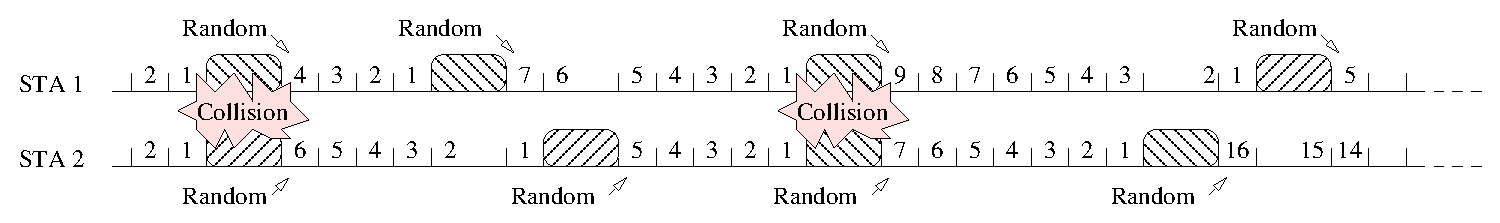
\includegraphics[width=5.5in]{figures/csma_ca}%
\label{fig:csma_ca}}
\subfigure[CSMA/ECA]{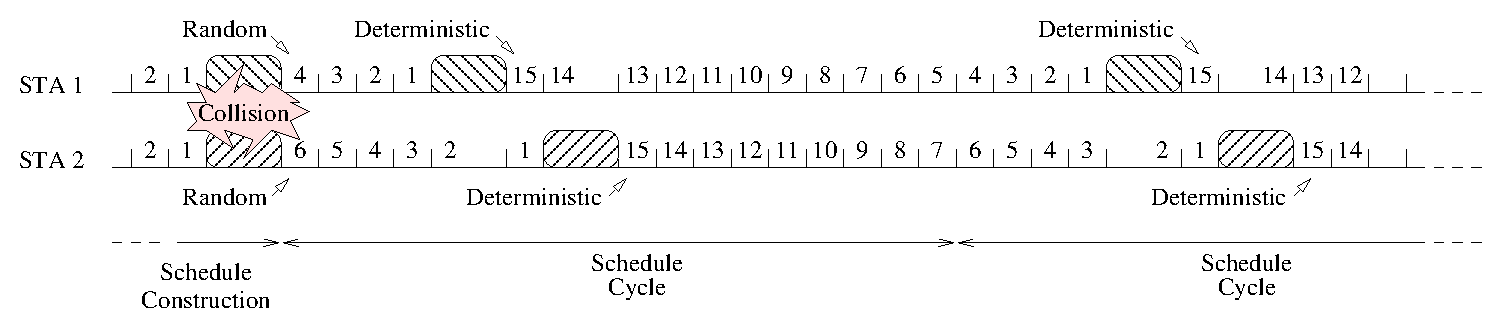
\includegraphics[width=5.5in]{figures/csma_eca}%
\label{fig:csma_eca}}
\caption{Examples of contention in which two wireless stations compete for channel access. The rounded boxes represent transmissions and the numbers are the backoff counters. It can be observed that CSMA/ECA attains cyclic collision-free operation after the construction of the schedule (transient convergence).}
\label{fig:ca_vs_eca}
\end{figure*}

Most of currently deployed WLANs are compliant with the IEEE 802.11 standard and rely on CSMA with collision avoidance (CSMA/CA) to share the channel time.
Thanks to the carrier sense capabilities of the CSMA stations, channel time can be divided in variable length slots.
%The stations take advantage of their carrier sense capabilities to divide channel time into variable length slots.
We classify the slots as either being empty, if no station transmits, or busy, if one or more stations transmit.
Among busy slots, we differentiate between successful slots, when there is a single transmission, and collision slots, when multiple stations simultaneously transmit.
Empty slots are relatively short and of constant duration, which is specified by the standard.
Contrastingly, busy slots are of variable length. 
Since the stations can use carrier sense to detect the end of a transmission, it is possible to synchronize the slots to the end of that variable length transmission.
The fact that the empty slots can be orders of magnitude shorter than the busy slots represents a performance gain over those approaches in which the slot size is fixed and constant.

In wired networks it is possible to use CSMA with collision detection (CSMA/CD) to keep the collision slots very short.
Contrastingly, wireless devices do not have the possibility to detect a collision while they are transmitting and, for this reason, the length of a collision slot is approximately equal to the length of the longest of the different packet transmissions involved in the collision.

The collision avoidance mechanism of CSMA/CA requires the stations to precede transmissions by a random backoff.
There is an exception to this rule: a station that joins the contention and senses the channel idle for an amount of time specified in the standard is allowed to immediately transmit.
Nevertheless, we can ignore this exception in our initial discussion and, for the sake of simplicity, assume that the stations always backoff for a random number of slots before transmitting.
In particular, the stations randomly choose a backoff value and set a backoff counter to that value.
Then, the stations decrement the backoff values by one in every slot.
The transmission occurs when the backoff counter reaches zero.

\subsection{The construction of a collisions-free schedule for two contending stations}
CSMA/ECA is simply a subtle variant of the protocol described above.
The only difference between CSMA/CA and CSMA/ECA is that the latter uses a deterministic backoff after successful transmissions.
This deterministic backoff is constant and is the same for all the stations.
As a result, two stations that successfully transmit in two different slots will not collide amongst themselves in their next transmission attempt.

%This is the key idea in CSMA/ECA and it is illustrated by the following example.
Imagine that two stations $STA1$ and $STA2$ successfully transmit in two different slots (for our example we will assume that these are slot $X$ and slot $Y$, respectively),  and then they both backoff for the same number of slots $V$.
Their next transmission attempt occurs at slot $X+V$ and $Y+V$, which are different (since $X$ and $Y$ are different).

The behaviour of CSMA/CA and CSMA/ECA is depicted in Fig.~\ref{fig:ca_vs_eca}.
The upper subfigure Fig. \ref{fig:csma_ca} represents two stations competing for the channel using CSMA/CA.
The channel time is slotted and some slots are empty while others are busy with successes or collisions.
The busy slots are in practice much longer than the empty ones, although the figure is not to scale for the ease of representation.
The figure also shows the backoff value of each of the two competing stations in each slot, and the tiny arrows indicate whether the backoff is randomly or deterministically selected.

It can be observed that the backoff value is decremented by one in every slot and that a station transmits when its backoff counter reaches a value equal to zero.
After a transmission, each CSMA/CA station randomly chooses a new backoff value.

In the present example we assume that, after completing a transmission, each station has another packet to transmit.
In the literature, this particular assumption is often referred to as saturation condition (e.g., \cite{he2009srb,barcelo2010fcc,fang2011dlm,barcelo2011tcf}).
We will keep the saturation assumption in the remainder of the paper, although in the next section we will mention references that address the non-saturation scenario.

The CSMA/CA stations in Fig.~\ref{fig:csma_ca} always use a random backoff, which means that they are always exposed to a collision probability greater than zero.
%
%A careful observation of the CSMA/CA example in the figure reveals that the stations do not make any effort to construct a collision free schedule.
%On the contrary, each station behaves randomly, making it impossible for the other station to make any prediction or gain any knowledge to reduce the chances of collision.
%As a result, CSMA/CA suffers from a high collision rate that undermines the overall network performance.
%The presence of collision slots is much more harmful than the presence of empty slots, since collision slots are much longer.
%In contrast to wired networks such as Ethernet, in WLANs it is not possible to detect the collision until the transmission is completed.
%Therefore, the colliding stations keep on transmitting the whole packet and the duration of the collision is equal to the duration of the longest of the transmissions involved in the collision.
It is useful to compare the behaviour of CSMA/CA in Fig. \ref{fig:csma_ca} to the behaviour of CSMA/ECA in Fig. \ref{fig:csma_eca}.
The initial behaviour is exactly the same for the two protocols: a collision occurs and a random backoff is selected.
However, after the first successful transmission of $STA 1$ we can observe that the CSMA/ECA station deterministically chooses its backoff value.
The same occurs after the first successful transmission of $STA 2$.
The fact that the stations have successfully transmitted in different slots and use the same deterministic backoff value guarantees that these two stations will not collide in their next transmission attempt.
%In fact, by choosing the same deterministic backoff, these two stations are in order to prevent a collision in the future.
From this point on, the behaviour of the system is collision-free, deterministic, cyclic and fair.
The cycle length is indicated in the figure, and it is easy to observe that the behaviour of the system in the second cycle is exactly the same as in the first cycle.

\subsection{Generalization to a larger number of contenders}
The general rule is that collision free operation is reached after all the contending stations consecutively successfully transmit.
To better understand the construction of the collision-free schedule, it is useful to look at an example with more than two contending stations.
In order to depict the contention for the channel when the number of contenders is high, we will need a more compact representation such as the used in Fig.~\ref{fig:ca_vs_eca_compact}.
For convenience, we draw all the slots as being of equal length, even though in reality their length can differ by orders of magnitude.
Each slot is numbered and the transmissions of the stations are represented as disks in the slots.
There are six different stations competing for the channel and the hatching pattern of each disk identifies which is the transmitting station.

\begin{figure*}[!t]
\centering
\subfigure[CSMA/CA]{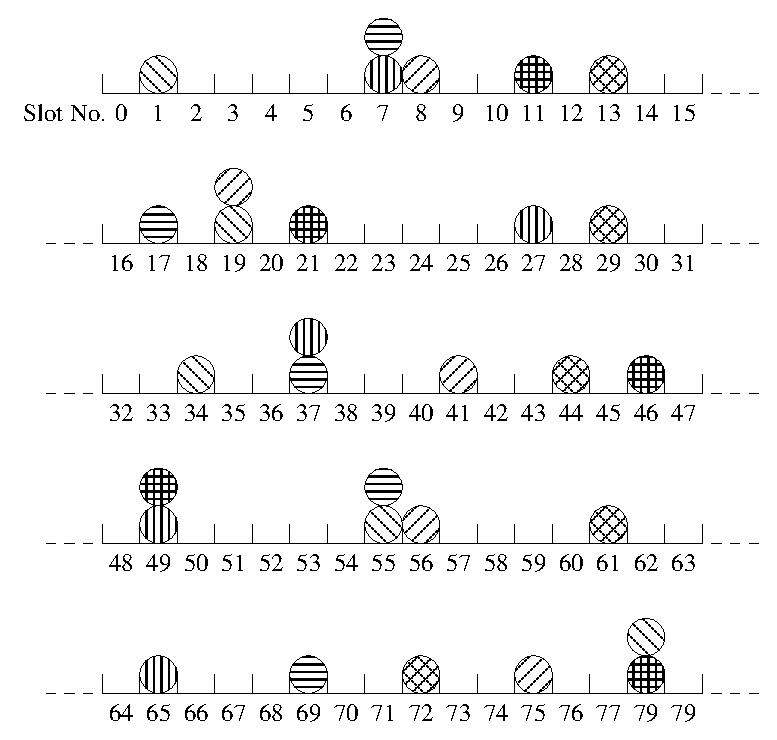
\includegraphics[width=2.5in]{figures/csma_ca_compact}%
\label{fig:csma_ca_compact}}
\subfigure[CSMA/ECA]{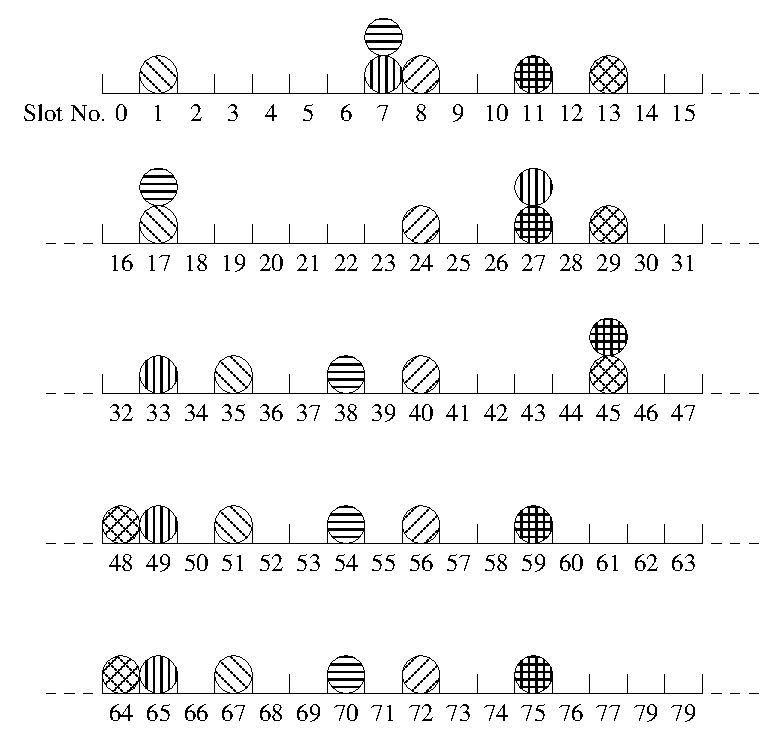
\includegraphics[width=2.5in]{figures/csma_eca_compact}%
\label{fig:csma_eca_compact}}
\caption{A compact representation of contention in which six wireless stations compete for channel access. The disks represent the transmissions of the stations and the  patterns are used to identify the station that transmitted. The construction of the collision-free schedule in CSMA/ECA finishes when all the stations consecutively successfully transmit.}
\label{fig:ca_vs_eca_compact}
\end{figure*}

%In CSMA/CA all the transmissions are preceded by a random backoff, and therefore no collision-free schedule is reached no matter how long the system runs.
%On the other hand, in CSMA/ECA the stations use a deterministic backoff after successful transmissions.
As in the previous example in Fig.~\ref{fig:csma_eca}, in the CSMA/ECA example in Fig.~\ref{fig:csma_eca_compact} the stations use a deterministic backoff after successful transmissions.
For convenience, the slots have been arranged in such a way that a deterministic backoff is represented by a new transmission in the same column of the following row.
As an example, the CSMA/ECA station that successfully transmits in slot 1 transmits again in slot 17, in the same column.
If we focus in the two CSMA/ECA stations that collide in slot 7, we realize that they use a random backoff which means that the new transmissions will probably end up in a different column.
In this particular example, the colliding stations in slot 7 retransmit in slot 17 and 27 respectively.
%Every time that a station suffers a collision, it uses a random backoff looking for an empty slot.
In CSMA/ECA, when all the stations consecutively successfully transmit, they all stick to the same column and the collision-free schedule has already been constructed.
This is exactly what we can observe in the last two rows of Fig. \ref{fig:csma_eca_compact}.

The construction of the collision-free schedule results in important performance gains in terms of throughput as we will see in the next section.
CSMA/ECA delivers a performance advantage even before the collision-free schedule is completely constructed.
This means that CSMA/ECA also outperforms CSMA/CA in highly dynamic scenarios in which the stations join and leave the contention.
In the extreme case in which the stations join the contention to transmit a single packet and then they leave, the performance of CSMA/ECA falls back to that of CSMA/CA.

A key aspect in the proposed protocol is that of the schedule length, which is equivalent to the deterministic backoff used after successful transmissions.
If the schedule length is excessively large compared to the number of contenders, the large number of empty slots will slightly penalize the performance.
On the other hand, if the schedule is too short, it would not be possible to accommodate the collision-free operation of all the participants.
As it is pointed out in \cite{fang2011dlm}, it is better to have a schedule that is larger than the number of contenders than having a one that it is shorter.
The reason is that empty slots are much shorter than collision slots.
We discuss in the next section the possibility to adapt the schedule length in a distributed way.

It is notable that the collision reduction and the performance improvement is obtained with no extra cost in terms of complexity, signaling or overhead.
%It is notable that the collisions are prevented without requiring any additional signaling or processing costs by part of the station.
Another advantage of CSMA/ECA is the close similarity to the protocol that is used in currently deployed devices, CSMA/CA.
This similarity should pave the way for the widespread implementation of CSMA/ECA in next-generation devices.

This section has covered the basic idea that enables the construction of a collision-free schedule in a highly idealized and simplified scenario. If CSMA/ECA is to be considered as a replacement of CSMA/CA, wider and deeper analysis are needed. The following section offers an overview of some contributions in this particular research area.

\section{Mathematical framework, performance evaluation and refinements}
\label{sec:survey}
%It is not the intention of this section to provide an exhaustive survey of all the contributions that deal with the construction of a collision-free schedule.
In this section we will comment on a small subset of contributions to offer an overview of some of the problems and enhancements of the basic idea that we have described in the previous section. 
Some of the issues we will be looking at are the underlying mathematical framework, backward compatibility, operation in the presence of errors and operation in networks with a very large number of contenders. 

\subsection{Underlying mathematical framework}
Even though CSMA/ECA was initially suggested to prevent collisions in WLANs, it has been recently shown that the underlying mathematical framework is applicable to disparate resource allocation problems in the field of networking, such as channel selection for channel spatial reuse and network coding \cite{duffy2011dcs}.
The construction of a collision-free schedule in CSMA/ECA is just an instance of a Constraint Satisfaction Problem (CSP) that the participating entities need to solve without explicit communication.
It is proven in \cite{duffy2011dcs} that the stochastic decentralized CSP solver that we have implicitly introduced in the previous section guarantees that a solution will be found in finite time, if the solution exists.
Furthermore, its performance is competitive with some of the well-known centralized CSP solvers.

\subsection{Refinements}

Some improvements on top of the basic idea described in Sec.~\ref{sec:eca} are presented in \cite{fang2011dlm}. 
First, it suggests a distributed approach to adjust the schedule length to accommodate a large number of contenders.
And second, it introduces the concept of stickiness, whereby the stations stick to a deterministic backoff even after a transmission failure, for increased schedule robustness. 
%We will take a closer look into these two contributions.

Notice that, if the protocol is used as described in the previous section, there is a maximum number of stations that can be accommodated in a collision-free fashion.
In other words, if there were more stations than columns in Fig. \ref{fig:csma_eca_compact}, it would not be possible to assign the stations to columns in such a way that there was a single station in each column.
This is the counting argument that is often referred to as the pigeonhole principle.
%If there are more pigeons than pigeonholes, then there is at least one pigeonhole with two pigeons.

Obviously, a mechanism that dynamically adjusted the number of columns (i.e., the value of the deterministic backoff after successes) as a function of the number of contending stations would solve the issue.
However, reaching this goal in a distributed fashion without requiring any kind of message exchange and preserving the system's fairness is quite a challenge.
The solution proposed in \cite{fang2011dlm} is simple and effective.
A station that perceives a high collision probability doubles the deterministic backoff that it uses after successful transmissions.

\begin{figure*}[!t]
\centering
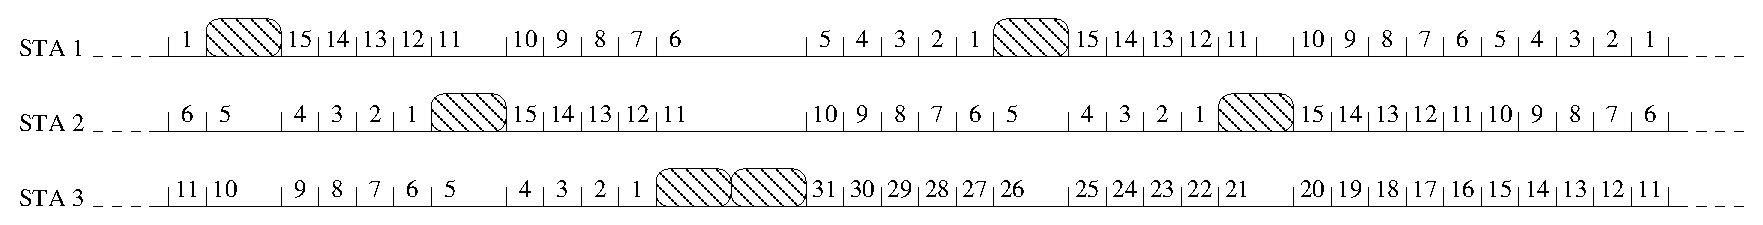
\includegraphics[width=6.0in]{figures/csma_eca_different_backoff}
\caption{Schedule length distributed adaption example. All the stations transmit the same number of packets in each cycle, despite using different schedule lengths.}
\label{fig:csma_eca_different_backoff}
\end{figure*}

The beautiful aspect of this approach is that the station that doubles its deterministic backoff also doubles the number of packets that are transmitted every time that it accesses the medium.
Using this trick, the number of available slots increases.
Remarkably, in the long term, all the stations transmit the same number of packets, independently of their schedule length.
This property makes it possible that different stations independently adjust their deterministic backoff value while fairness is preserved.

This approach can be better understood by means of an example.
Consider Fig. \ref{fig:csma_eca_different_backoff} in which three stations have reached a collision-free schedule.
Notice that the schedule length of the bottom station is twice as long as the schedule length of the other two stations.
Nevertheless, all the stations fairly share the channel, since the stations with short schedules transmit a single packet and the station with the long schedule transmits two packets when it is its turn.
Transmitting more than one packet when accessing the channel is possible and the latest revision of the IEEE 802.11 standard includes the necessary mechanisms for transmitting two or more packets back-to-back.
At the end of the large cycle of 32 slots, all the stations have transmitted two packets.

%The idea of stickiness, in the sense that a station is likely to keep using a deterministic backoff (even after a transmission failure) if it has been using a deterministic backoff for a few times in a row, provides the protocol with some extra robustness in the case of a channel error or the entry of a new contender. 
%Notice that either one of these two events, can force a station to switch from a deterministic backoff to a random backoff.
%This change can easily result in more collisions, triggering a cascading effect in which multiple stations switch to a random backoff and they have to construct a new schedule.
%If a station sticks to a deterministic backoff after a transmission failure, it is less likely that a channel error or a new entrant disrupts the collision-free operation.
%An additional advantage of stickiness is that it reduces the time that is required to construct the collision-free schedule.
%We refer the interested reader to the original paper \cite{fang2011dlm} for details about the choice of the sticking probability.

\begin{figure}[!t]
\centering
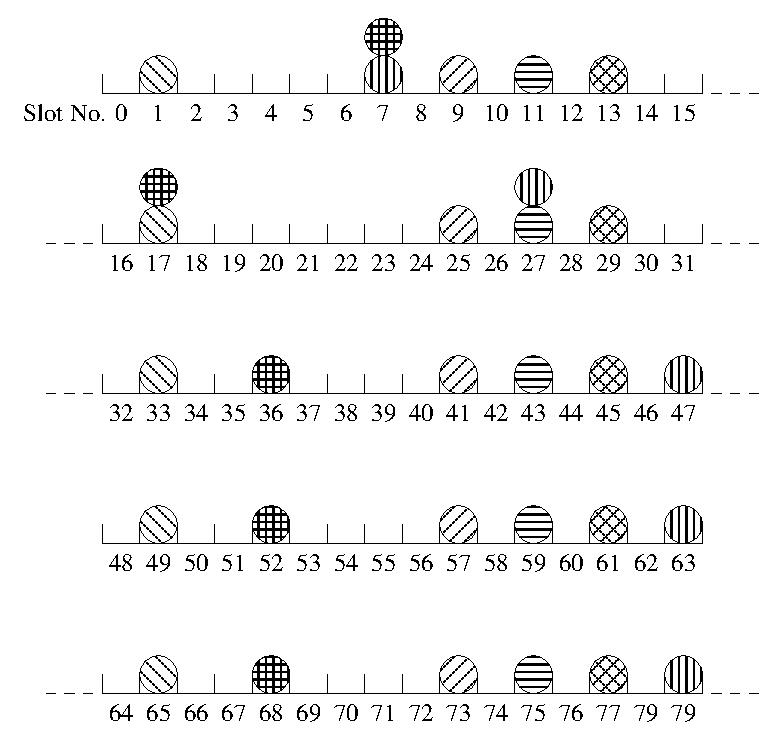
\includegraphics[width=2.5in]{figures/csma_e2ca}
\caption{The use of a deterministic backoff for two consecutive times after each successful transmission (CSMA/E2CA) speeds up the construction of the collision-free schedule.}
\label{fig:csma_e2ca}
\end{figure}


%A different approach to stickiness is presented in \cite{barcelo2011tcf}, where  CSMA/E2CA is introduced. 
%CSMA/E2CA is a variant of CSMA/ECA in which a deterministic backoff is used for two consecutive times after each successful packet transmission.
%Note that while the approach to stickiness in \cite{fang2011dlm} is probabilistic, in CSMA/E2CA it is deterministic.
%This deterministic nature can be appealing for manufacturers, since it simplifies the implementation.
%CSMA/E2CA also provides all the advantages that come with stickiness: shorter convergence time and further schedule resistance to channel errors and new entrants.

If CSMA/ECA is used as described in Sect.~\ref{sec:eca}, the entry of a new contender or a single channel error can disrupt collision-free operation.
To address this problem, stickiness was introduced in \cite{fang2011dlm} and later discussed in \cite{barcelo2011tcf} in a protocol called CSMA/E2CA.
In CSMA/E2CA, a station sticks to the use of a deterministic backoff for two consecutive times after each successful transmission.
In other words, a station that is using a deterministic backoff will only switch to a random behaviour if it suffers two contiguous unsuccessful transmissions.

The operation of CSMA/E2CA is illustrated in Fig. \ref{fig:csma_e2ca}.
In this figure, there is a station that successfully transmits in slot~11.
This station uses a deterministic backoff (i.e., sticks to the same column in this particular graphical representation) and then it suffers a collision in its next transmission attempt in slot 27.
Despite the collision, this station keeps using a deterministic backoff because the CSMA/E2CA protocol states that a deterministic backoff is used for two consecutive times after a successful transmission.
As a result, the station sticks to the same column avoiding collisions with other stations that have successfully transmitted.
Compare this behaviour to the behaviour observed in Fig. \ref{fig:csma_eca_compact} where the station that successfully transmits in slot 11, suffers a collision in slot 27 and then causes another collision after using a random backoff and transmitting in slot 45.

\subsection{Performance of CSMA/ECA and CSMA/E2CA}

A detailed study of the use of a deterministic backoff after successful transmissions is offered in \cite{he2009srb}. 
One the characteristics of the construction of the collision-free schedule is that it requires some time.
The network goes through a transient state in which some of the stations use a deterministic backoff while the remaining stations use a random backoff.
When the collision-free schedule is eventually reached, the system moves to a deterministic steady state.
An analytical model of the system is presented which can be used to make predictions about the length of transient state.

The paper also presents a comprehensive simulation study which includes realistic ingredients such as traffic differentiation, carrier sense errors and channel errors.
Different performance metrics such as throughput, delay and collision probability are evaluated and both saturated and non-saturated traffic is considered.
The authors conclude that the variant of the protocol that uses a deterministic backoff after successful transmissions always outperforms the purely random protocol.
Another interesting remark of that paper is the fact that the implementation of the protocol in the well-known simulator NS-2 required the change of only three lines of code.
This gives an idea of how similar the protocol is to the legacy one and how easy it would be to include the approach in new devices.

Fairness of the new protocol with regard to legacy stations is addressed in \cite{barcelo2010fcc}.
The results show that both protocols are interoperable and can fairly coexist in the same network.
CSMA/ECA stations will experience a slightly better performance than CSMA/CA stations, and the participation of legacy stations prevents the construction of a collision-free schedule.
Nevertheless, it is remarkable that the mix of new and legacy stations attains a better performance than a network in which all the stations follow the legacy protocol.

Backward compatibility is of paramount importance for any improvement to be adopted in WLANs, since there is a large base of deployed hardware that will not be thrown away overnight.
The possibility of CSMA/ECA to peacefully coexist with the previous protocol ensures a smooth transition from one protocol to the other, with a coexistence period in which both protocols will interoperate.

\begin{figure}[!t]
\centering
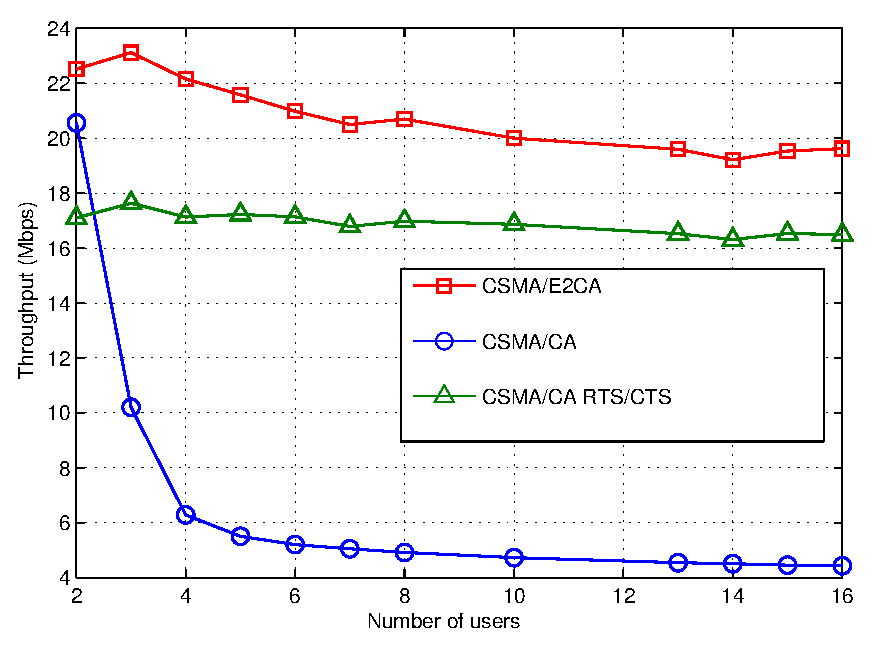
\includegraphics[width=\linewidth]{figures/performance}
\caption{The figure compares the analytical and simulation performance curves of CSMA/CA and CSMA/E2CA for an increasing number of contenders.}
\label{fig:performance}
\end{figure}

A detailed performance evaluation of the new protocol is offered in \cite{martorell2012pec}.
This paper presents an analytical model and simulations that use realistic channel realizations and the automated rate fallback (ARF) mechanism for the selection of the modulation coding scheme (MCS).
An exponentially packet length distribution is considered and the curves that compare CSMA/CA and CSMA/E2CA (See Fig.~\ref{fig:performance}) show a substantial goodput improvement, for both the basic access (BA) and the request-to-send/clear-to-send (RTS/CTS) scheme.


\section{Conclusion} \label{sec:conclusion}
In this paper we have presented a tutorial description of CSMA/ECA, a wireless MAC protocol in which the participating devices construct a collision-free schedule.
An interesting property is that this collaboration neither requires additional processing costs nor message interchange.
All that is needed, is that the stations use a deterministic backoff after successful transmissions.

By doing so, it is guaranteed that two stations that successfully transmitted in their last transmission attempt will not collide among them in their next transmission attempt.
Furthermore, in ideal conditions, the system will reach a steady-state in which all the stations transmit in a round-robin fashion in a collision-free schedule.

Obviously, those ideal conditions are not always satisfied, and in the second part of the paper we have reviewed different contributions that either assess the performance of the system in those non-ideal conditions or suggest improvements to deal with the non-idealities.
We have discussed the distributed adjustment of the schedule length to accommodate a potentially large number of contenders in a collision-free fashion.
And we have also introduced stickiness, which reduces the time required to construct the collision-free schedule and increases the robustness of the schedule in scenarios with channel errors or new stations joining the channel.

As a summary, we have provided an overview of a promising approach that could substantially reduce the problem of collisions in next generation WLANs.



% An example of a floating figure using the graphicx package.
% Note that \label must occur AFTER (or within) \caption.
% For figures, \caption should occur after the \includegraphics.
% Note that IEEEtran v1.7 and later has special internal code that
% is designed to preserve the operation of \label within \caption
% even when the captionsoff option is in effect. However, because
% of issues like this, it may be the safest practice to put all your
% \label just after \caption rather than within \caption{}.
%
% Reminder: the "draftcls" or "draftclsnofoot", not "draft", class
% option should be used if it is desired that the figures are to be
% displayed while in draft mode.
%
%\begin{figure}[!t]
%\centering
%\includegraphics[width=2.5in]{myfigure}
% where an .eps filename suffix will be assumed under latex, 
% and a .pdf suffix will be assumed for pdflatex; or what has been declared
% via \DeclareGraphicsExtensions.
%\caption{Simulation Results}
%\label{fig_sim}
%\end{figure}

% Note that IEEE typically puts floats only at the top, even when this
% results in a large percentage of a column being occupied by floats.


% An example of a double column floating figure using two subfigures.
% (The subfig.sty package must be loaded for this to work.)
% The subfigure \label commands are set within each subfloat command, the
% \label for the overall figure must come after \caption.
% \hfil must be used as a separator to get equal spacing.
% The subfigure.sty package works much the same way, except \subfigure is
% used instead of \subfloat.
%
%\begin{figure*}[!t]
%\centerline{\subfloat[Case I]\includegraphics[width=2.5in]{subfigcase1}%
%\label{fig_first_case}}
%\hfil
%\subfloat[Case II]{\includegraphics[width=2.5in]{subfigcase2}%
%\label{fig_second_case}}}
%\caption{Simulation results}
%\label{fig_sim}
%\end{figure*}
%
% Note that often IEEE papers with subfigures do not employ subfigure
% captions (using the optional argument to \subfloat), but instead will
% reference/describe all of them (a), (b), etc., within the main caption.


% An example of a floating table. Note that, for IEEE style tables, the 
% \caption command should come BEFORE the table. Table text will default to
% \footnotesize as IEEE normally uses this smaller font for tables.
% The \label must come after \caption as always.
%
%\begin{table}[!t]
%% increase table row spacing, adjust to taste
%\renewcommand{\arraystretch}{1.3}
% if using array.sty, it might be a good idea to tweak the value of
% \extrarowheight as needed to properly center the text within the cells
%\caption{An Example of a Table}
%\label{table_example}
%\centering
%% Some packages, such as MDW tools, offer better commands for making tables
%% than the plain LaTeX2e tabular which is used here.
%\begin{tabular}{|c||c|}
%\hline
%One & Two\\
%\hline
%Three & Four\\
%\hline
%\end{tabular}
%\end{table}


% Note that IEEE does not put floats in the very first column - or typically
% anywhere on the first page for that matter. Also, in-text middle ("here")
% positioning is not used. Most IEEE journals use top floats exclusively.
% Note that, LaTeX2e, unlike IEEE journals, places footnotes above bottom
% floats. This can be corrected via the \fnbelowfloat command of the
% stfloats package.



%\section{Conclusion}
%The conclusion goes here.





% if have a single appendix:
%\appendix[Proof of the Zonklar Equations]
% or
%\appendix  % for no appendix heading
% do not use \section anymore after \appendix, only \section*
% is possibly needed

% use appendices with more than one appendix
% then use \section to start each appendix
% you must declare a \section before using any
% \subsection or using \label (\appendices by itself
% starts a section numbered zero.)
%


%\appendices
%\section{Proof of the First Zonklar Equation}
%Appendix one text goes here.

% you can choose not to have a title for an appendix
% if you want by leaving the argument blank
%\section{}
%Appendix two text goes here.


% use section* for acknowledgement
%\section*{Acknowledgment}


%The authors would like to thank...


% Can use something like this to put references on a page
% by themselves when using endfloat and the captionsoff option.
%\ifCLASSOPTIONcaptionsoff
%  \newpage
%\fi



% trigger a \newpage just before the given reference
% number - used to balance the columns on the last page
% adjust value as needed - may need to be readjusted if
% the document is modified later
%\IEEEtriggeratref{8}
% The "triggered" command can be changed if desired:
%\IEEEtriggercmd{\enlargethispage{-5in}}

% references section

% can use a bibliography generated by BibTeX as a .bbl file
% BibTeX documentation can be easily obtained at:
% http://www.ctan.org/tex-archive/biblio/bibtex/contrib/doc/
% The IEEEtran BibTeX style support page is at:
% http://www.michaelshell.org/tex/ieeetran/bibtex/
\bibliographystyle{IEEEtran}
% argument is your BibTeX string definitions and bibliography database(s)
\bibliography{IEEEabrv,my_bib}
%
% <OR> manually copy in the resultant .bbl file
% set second argument of \begin to the number of references
% (used to reserve space for the reference number labels box)
%\begin{thebibliography}{1}

%\bibitem{IEEEhowto:kopka}
%H.~Kopka and P.~W. Daly, \emph{A Guide to \LaTeX}, 3rd~ed.\hskip 1em plus
%  0.5em minus 0.4em\relax Harlow, England: Addison-Wesley, 1999.

%\end{thebibliography}

% biography section
% 
% If you have an EPS/PDF photo (graphicx package needed) extra braces are
% needed around the contents of the optional argument to biography to prevent
% the LaTeX parser from getting confused when it sees the complicated
% \includegraphics command within an optional argument. (You could create
% your own custom macro containing the \includegraphics command to make things
% simpler here.)
%\begin{biography}[{\includegraphics[width=1in,height=1.25in,clip,keepaspectratio]{mshell}}]{Michael Shell}
% or if you just want to reserve a space for a photo:

%\begin{IEEEbiography}{Michael Shell}
%Biography text here.
%\end{IEEEbiography}

% if you will not have a photo at all:
%\begin{IEEEbiographynophoto}{John Doe}
%Biography text here.
%\end{IEEEbiographynophoto}

% insert where needed to balance the two columns on the last page with
% biographies
%\newpage

%\begin{IEEEbiographynophoto}{Jane Doe}
%Biography text here.
%\end{IEEEbiographynophoto}

% You can push biographies down or up by placing
% a \vfill before or after them. The appropriate
% use of \vfill depends on what kind of text is
% on the last page and whether or not the columns
% are being equalized.

%\vfill

% Can be used to pull up biographies so that the bottom of the last one
% is flush with the other column.
%\enlargethispage{-5in}



% that's all folks
\end{document}


